% % % % % % % % % % % % % % % % % % % % % % % % % % % % % % % % % % % % % % % % 
% Formelsammlung von LaTeX4EI									
%
% @encode: 	UTF-8, tabwidth = 4, newline = LF
% @author:	Lukas Kompatscher, Emanuel Regnath (orginal HM3 und HM4)
% @date:		
%
% % % % % % % % % % % % % % % % % % % % % % % % % % % % % % % % % % % % % % % % 

%---------------------------------------%
%				Analysis 3				%
%~~~~~~~~~~~~~~~~~~~~~~~~~~~~~~~~~~~~~~~%

% Document Class ===============================================================
\documentclass[german,color]{latex4ei/latex4ei_fs}

% set document information
\title{Analysis 3}
\author{Lukas Kompatscher (LaTeX4EI)}	
\myemail{info@latex4ei.de}	


% DOCUMENT_BEGIN ===============================================================
\begin{document}

\maketitle

% SECTION ======================================================================
\section{Nützliches Wissen $e^{\i x} = \cos (x) + \i \cdot \sin(x)$}
% ==============================================================================
\begin{sectionbox}
	\subsection{Sinus, Cosinus \quad $\sin^2(x) \bs + \cos^2(x) = 1$}
	%noneed \setlength{\tabcolsep}{4pt}
	\begin{tablebox}{c|c|c|c|c||c|c|c|c}
	$x$ & $0$ & $\pi / 6$ & $\pi / 4$ & $\pi / 3$ & $\frac{1}{2}\pi$ & $\pi$ & $1\frac{1}{2}\pi$ & $2 \pi$ \\
	$\scriptstyle{ \varphi }$ & $\scriptstyle{0^\circ}$ & $\scriptstyle{30^\circ}$ & $\scriptstyle{45^\circ}$ & $\scriptstyle{60^\circ}$ & $\scriptstyle{90^\circ}$ & $\scriptstyle{180^\circ}$ & $\scriptstyle{270^\circ}$ & $\scriptstyle{360^\circ}$ \\ \cmrule
	$\sin$ & $0$ & $\frac{1}{2}$ & $\frac{1}{\sqrt{2}}$ & $\frac{\sqrt 3}{2}$ & $1$ & $0$ & $-1$ & $0$ \\
	$\cos$ & $1$ & $\frac{\sqrt 3}{2}$ & $\frac{1}{\sqrt 2}$ & $\frac{1}{2}$ & $0$ & $-1$ & $0$ & $1$ \\     
	$\tan$ & $0$ & $\frac{\sqrt{3}}{3}$ &	$1$	&	$\sqrt{3}$ & $\pm \infty$ & $0$ & $\mp \infty$ & $0$\\ 
	\end{tablebox}
	\begin{tablebox}{ll}
		Additionstheoreme &  Stammfunktionen\\
	 	$\cos (x - \frac{\pi}{2}) = \sin x$ & $\int x \cos(x) \diff x = \cos(x) + x \sin(x)$\\
	 	$\sin (x + \frac{\pi}{2}) = \cos x$ & $\int x \sin(x) \diff x = \sin(x) - x \cos(x)$\\
	 	$\sin 2x = 2 \sin x \cos x $  & $\int \sin^2(x) \diff x = \frac12 \bigl(x - \sin(x)\cos(x) \bigr)$\\ 
	 	$\cos 2x = 2\cos^2 x - 1$  & $\int \cos^2(x) \diff x = \frac12 \bigl(x + \sin(x)\cos(x) \bigr)$\\
	 	$\sin(x) = \tan(x)\cos(x)$ & $\int \cos(x)\sin(x) = -\frac12 \cos^2(x)$ \\
	\end{tablebox}
		\textbf{Sinus/Cosinus Hyperbolicus} $\sinh, \cosh$\\ 
		% \quad \operatorname{arsinh}\ x:= \ln\left(x+\sqrt{x^2+1}\right) \\
		\begin{tabular*}{\columnwidth}{@{\extracolsep\fill}ll@{}}
		$\sinh x = \frac{1}{2}(e^x -e^{-x})= - \i \, \sin(\i x)$ & $\cosh^2 x  \bs - \sinh^2 x = 1$\\
		$\cosh x  = \frac{1}{2}(e^x +e^{-x})= \cos(\i x)$ & $\cosh x + \sinh x = e^{x}$\\
		\end{tabular*}\\
		\textbf{Kardinalsinus} $\mathrm{si}(x) = \frac{\sin(x)}{x}$ \qquad genormt: $\sinc(x) = \frac{\sin(\pi x)}{\pi x}$
\end{sectionbox}

\begin{sectionbox}
	\subsection{Integrale $\int e^x\;\mathrm{d} x = e^x = (e^x)'$}
	Partielle Integration: $\int uw'=uw-\int u'w$\\
	Substitution: $\int f(g(x)) g'(x)\,\mathrm dx=\int f(t)\, \mathrm dt$\\
	\renewcommand{\arraystretch}{1.6} 
	\begin{tablebox}{ccc}
		$F(x)$ & $f(x)$ & $f'(x)$ \\ \cmrule
		$\frac{1}{q+1}x^{q+1}$ & $x^q$ & $qx^{q-1}$ \\
		\raisebox{-0.2em}{$\frac{2\sqrt{ax^3}}{3}$} & $\sqrt{ax}$ & \raisebox{0.2em}{$\frac{a}{2\sqrt{ax}}$}\\
		$x\ln(ax) -x$ & $\ln(ax)$ & $\textstyle \frac{a}{x}$\\
		%e^x & e^x & e^x \\
		$\frac{1}{a^2} e^{ax}(ax- 1)$ & $x \cdot e^{ax}$ & $e^{ax}(ax+1)$ \\
		$\frac{a^x}{\ln(a)}$ & $a^x$ & $a^x \ln(a)$ \\
		$-\cos(x)$ & $\sin(x)$ & $\cos(x)$\\
		$\cosh(x)$ & $\sinh(x)$ & $\cosh(x)$\\
		$-\ln |\cos(x)|$ & $\tan(x)$ & $\frac{1}{\cos^2(x)}$ \\
	\end{tablebox}
	
	$\int e^{at} \sin(bt) \diff t = e^{at} \frac{a \sin(bt) + b \cos(bt)}{a^2 + b^2}$\\
	\begin{tablebox}{ll}
		$\int \frac{\diff t}{\sqrt{at+b}} = \frac{2 \sqrt{at+b}}{a}$ & $\int t^2 e^{at} \diff t = \frac{(ax-1)^2+1}{a^3} e^{at}$\\
		$\int t e^{at} \diff t = \frac{at-1}{a^2} e^{at}$ & $\int x e^{ax^2} \diff x = \frac{1}{2a} e^{ax^2}$\\
	\end{tablebox}
\end{sectionbox}

\begin{sectionbox}
	\subsection{Exponentialfunktion und Logarithmus $e^0=e^{\i2\pi}=1$}
	\begin{tabular}{lll}
		$a^x = e^{x \ln a}$ & $\log_a x = \frac{\ln x}{\ln a}$ & $\ln x \le x -1$\\
		$\ln(x^{a}) = a \ln(x)$ & $\ln(\frac{x}{a}) = \ln x - \ln a$ & $\log(1) = 0$\\
	\end{tabular}
\end{sectionbox}

\begin{sectionbox}
	\subsection{Imaginäre Einheit}
	$\i = \sqrt{-1}$ \qquad $|\cx z|^2 = \cx z \cxc z = x^2+y^2$
\end{sectionbox}

\begin{sectionbox}
	\subsection{Reihen}
	$\underset{\text{Harmonische Reihe}}{\sum\limits_{n=1}^\infty \frac{1}{n} \ra \infty} \qquad   \underset{\text{Geometrische Reihe}}{\sum\limits_{n=0}^\infty q^n \stackrel{|q|<1}= \frac{1}{1-q}}  \qquad \underset{\text{Exponentialreihe}}{\sum\limits_{n = 0}^{\infty} \frac{z^n}{n!} = e^z}$
\end{sectionbox}

\begin{sectionbox}
	\subsection{Wichtige Formeln}
	%noneed \setlength{\tabcolsep}{0pt}
	
	\begin{tablebox}{ll}
			Dreiecksungleichung: &$\big|\! \abs{x}- \abs{y}\!\big| \le \abs{x \pm y} \le \abs{x} + \abs{y}$\\
			Cauchy-Schwarz-Ungleichung: & $\left| \vec x^\top \bdot \vec y \right| \le \| \vec x\| \cdot \| \vec y\|$ \\
			Bernoulli-Ungleichung: & $(1+x)^n \ge 1+nx$\\ \cmrule
			Aritmetrische Summenformel &  $\sum \limits_{k=1}^{n} k = \frac{n (n+1)}{2} $ \\
			Geometrische Summenformel &  $ \sum \limits_{k=0}^{n} q^k = \frac{1 - q^{n+1}}{1-q}$ \\
			Binomialkoeffizient & $\binom nk = \binom n{n-k} = \frac{n!}{k! \cdot (n-k)!}$\\
	\end{tablebox}
\end{sectionbox}
	

% SECTION ======================================================================
\section{Fourierreihe}
% ==============================================================================
\begin{sectionbox}
ist die Entwicklung einer Funktion $f\in C(T)$ in eine Reihe aus $\sin$ und $\cos$.\\
$C(T):$ \emph{$T$-periodisch, stetig fortsetzbar}\\
$f$ ist $T$-periodisch, falls $f(x+T) = f(x)$ $\ra$ auch $n \cdot T$ periodisch.

	\begin{cookbox}{Entwicklung in Fourierreihen $f(x) \sim S_f(x)$}
		\item Bestimme die Fourierkoeffizienten zu $f \in C(T)$:\\
		$a_k,b_k \in \R$: \quad \boxed{ \Big\{ { ^{\textstyle a_k}_{\textstyle b_k}} = \frac{2}{T} \int\limits_{-\frac{T}{2}}^{\frac{T}{2}} f(x) \Big\{ {}^{\textstyle \cos} _{\textstyle \sin} \left(k \frac{2\pi}{T} x \right) \diff x }\\
		\emph{$a_0$ immer separat berechnen mit $k = 0$!}\\
		$c_k \in \C$: \quad \boxed{ c_k = \frac{1}{T} \int\limits_{-\frac{T}{2}}^{\frac{T}{2}} f(x) \exp \left( - \i k \frac{2 \pi}{T} x \right) \diff x } \\
		\emph{$c_0$ immer separat berechnen mit $k = 0$!}\\
		
		\item Aufstellen der Fourierreihe $S_f$ zu $f$:  \\
		\boxed{ S_f(x) = \frac{a_0}{2} + \sum\limits_{k=1}^\infty a_k \cos \left(k \frac{2\pi}{T} x \right) + b_k \sin \left( k \frac{2\pi}{T} x \right) } \\
		\boxed{ S_f(x) = \sum\limits_{k=-\infty}^\infty c_k \exp \left( \i k \frac{2 \pi}{T} x \right) }
	\end{cookbox}
	
	\emph{Konvergenz:} $S_f(x) \sim f(x)$ \ $\Ra$ \ $f$ in $x$ \emph{stetig \& stückweise stetig differenzierbar} $\Ra$ $S_f(x) = f(x)$\\
	$f$ nicht in $x$ stetig $\Ra$ $x = a_i$ und $S_f(x) = \frac{f(a_i^+) + f(a_i^-)}{2}$\\
\end{sectionbox}

\begin{sectionbox}
	\subsection{Rechenregeln}
	\begin{tablebox}{ll}
		Linearität & $\alpha f + \beta g \FT \alpha c_k + \beta d_k$\\
		Konjugation & $\ol{f} \FT \ol{c_{-k}}$\\
		Zeitumkehr & $f(-t) \FT c_{-k}$\\
		Streckung & $f(\gamma t) \FT c_k; \gamma > 0; \tilde{T} = \frac{T}{\gamma}$\\
		Verschiebung $t$ & $f(t + a) \FT e^{\i k \omega a} c_k$\\
		Verschiebung $\omega$ & $e^{\i n \omega t} f(t) \FT c_{k - n}$\\
		Ableitung & $\dot{f}(t) \FT \i k \omega c_k$\\
		Stammfunktion & $\int_0^t f(t) \FT \begin{cases} \frac{c_k}{\i k \omega} & k \neq 0\\ -\frac{1}{T}\int_0^T t f(t) \diff t & k = 0\\ \end{cases}$\\
		& $c_{0_{f(t)}} \stackrel{!}{=} 0$\\
		Faltung & $f * g \FT c_k d_k$\\
	\end{tablebox}
\end{sectionbox}

\begin{sectionbox}
	\subsection{Symmetrien}
	\begin{itemize}
		\item $f$ gerade (achsensym.) Funktion: $f(t) = f(-t)$\\
		$c_k = c_{-k}$\\
		$b_k = 0$ \qquad $a_k = \frac{4}{T} \int_{0}^{T/2} f(x) \cos \left(k \frac{2\pi}{T} x \right) \diff x$
		\item $f$ ungerade (punktsym.) Funktion: $f(t) = -f(-t)$\\
		$c_k = -c_{-k}$\\
		$a_k = 0$ \qquad $ b_k = \frac{4}{T} \int_{0}^{T/2} f(x) \sin \left(k \frac{2\pi}{T} x \right) \diff x$
		\item $f$ $\frac{T}{2}$-periodisch: $f(\frac{T}{2} + t) = f(t)$\\
		$c_{2k+1} = a_{2k+1} = b_{2k+1} = 0$\\
		$\begin{cases} a_{2k}\\ b_{2k} \end{cases} = \frac{1}{T}\int_0^{T/2}f(t)\begin{cases} \cos{(2k \omega t)}\\ \sin{(2k \omega t)} \end{cases} \diff t$
		\item $f$ ohne $\frac{T}{2}$-periodischen Anteil: $f(\frac{T}{2} + t) = -f(t)$\\
		$c_{2k} = a_{2k} = b_{2k} = 0$\\
		$\begin{cases} a_{2k+1}\\ b_{2k+1} \end{cases} = \frac{1}{T}\int_0^{T/2}f(t)\begin{cases} \cos{((2k+1) \omega t)}\\ \sin{((2k+1) \omega t)} \end{cases} \diff t$
	\end{itemize}
\end{sectionbox}

\begin{sectionbox}
	\subsection{Umrechnungsformeln}
	\begin{itemize}
		\item $a_0 = 2 c_0 \quad a_k = c_k + c_{-k}$  \quad $b_k = \i (c_k - c_{-k})$
		\item $c_0 = \frac{a_0}{2} \quad c_k = \frac12(a_k - \i b_k) \quad c_{-k} = \frac12(a_k + \i b_k)$
	\end{itemize}
\end{sectionbox}

\begin{sectionbox}
	\subsection{LTI-Systeme}
	$L[y](t) = a_n y^{(n)}(t) + \cdots + a_1 \dot{y}(t) + a_0 y(t) = x(t)$\\
	$\frac{\diff^n}{\diff t^n} \ra s^n \ra P(s) = a_n s^n \cdots + a_1 s + a_0$\\
	$h_T(t) = \sum_{k=-\infty}^{\infty}d_k e^{\i k \omega t}$ mit $d_k = \frac{1}{P(\i k \omega)}$\\
	$y(t) = h_T(t)*x(t) = \int_0^T h_T(\tau) x(t - \tau) \diff \tau$
\end{sectionbox}

\begin{sectionbox}
	\subsection{Umrechnung von $T$ in $S$ periodische Funktionen}
	$f$ ist $T$ periodisch, $g(x) = f\left( \frac{T}{S} x \right)$, $S$ periodisch, denn
	$g(x+S) = f\left( \frac{T}{S} (x+S) \right) = f\left( \frac{T}{S} x + T \right) = f\left( \frac{T}{S} x \right) = g(x)$\\
\end{sectionbox}

\begin{sectionbox}
	\subsection{Funktionen}
	\subsubsection{Sägezahnfunktion}
	$s(t) = \frac{1}{2}(\pi - t), \quad 0 < t < 2 \pi, \quad T = 2 \pi, \quad \omega = 1$\\
	$c_0 = 0; \qquad c_k = \frac{1}{2k \i}$\\
	$S_f(t) = \sum_{k=1}^{\infty}\frac{1}{k}\frac{e^{\i k t} - e^{-\i k t}}{2 \i}$
\end{sectionbox}


% SECTION ======================================================================
\section{Fouriertransformation $f(t) \ra F(\omega)$}
% ==============================================================================
\begin{sectionbox}
	\emph{Voraussetzungen:}
	\begin{enumerate}
		\item $f$ stückweise stetig differenzierbar
		\item $f(t) = \frac{1}{2}\left(f(t^+) + f(t^-)\right)$
		\item $\int_{-\infty}^{\infty}\abs{f(t)} \diff t < \infty$ ($f$ absolut integrierbar)
	\end{enumerate}
	\quad \\
	$f \ra F$ mit Zeitfunktion $f:\R \ra \C$ und Frequenzfkt./Spektralfkt $F$\\
	%Es muss gelten: $\lim\limits_{t \ra \pm \infty} f(t) = 0$ \quad $f$ fourtransbar, falls \\
	\boxed{ F(\omega) := \int\limits_{-\infty}^\infty f(t) \exp(-\i \omega t) \diff t} \\
	
	Wichtige Fouriertransformationen:\\
	\begin{tabular}{rl|rl}
		$f(t)$ & \qquad $F(\omega)$ & $f(t)$ & \qquad $F(\omega)$\\		%Graph mit zwei Farben?
		$1$ & \!\!\!\!\!\!\!\!\!\! $\LT 2\pi \delta(\omega)$ & $|t^n|$ & \!\!\!\!\!\!\!\!\!\! $\LT \frac{2n!}{(\i \omega)^{n+1}}$\\
		$t^n$ & \!\!\!\!\!\!\!\!\!\! $\LT 2\pi \i^n \delta^{(n)}(\omega)$ & $\frac{t^{n-1}}{(n-1)!} e^{-at} u(t)$ & \!\!\!\!\!\!\!\!\!\! $\LT \frac{1}{(a+\i \omega)^n}$\\
		$\heavi(t)$ & \!\!\!\!\!\!\!\!\!\! $\LT \frac{1}{\i \omega} + \pi \delta(\omega)$ & $\delta(t-t_0)$ & \!\!\!\!\!\!\!\!\!\! $\LT e^{-\i \omega t_0}$
	\end{tabular}
	\subsection{Die Inverse Fouriertransformation}
	$f(t) = \frac{1}{2\pi} \int\limits_{-\infty}^\infty F(\omega) \exp(\i \omega t) \diff \omega$\\
	$\begin{cases} f(t) & ,f\ \text{ stetig in }t \\ \frac{f(t^-) + f(t^+)}{2} & ,\text{falls } f\text{ unstetig in }t \end{cases}$
\end{sectionbox}

\begin{sectionbox}
	\subsection{Die Dirac'sche Deltafkt. $\delta(t)$}
	$\delta_\varepsilon(t-t_0) = \frac{1}{\varepsilon}$, für $t_0 \le t \le t_0 + \varepsilon$, sonst $0$\\
	Für stetiges $g$ gilt: $\int_{-\infty}^\infty g(t) \delta(t-t_0) \diff t = g(t_0)$\\
	$\Delta_{t_0} (\omega) = \int_{-\infty}^\infty \delta(t-t_0) \exp(-\i \omega t) \diff t = \exp(-\i \omega t_0)$\\
	$\delta(t-t_0) \LT \Delta_{t_0} (\omega)$ und $\delta(t) \LT 1$
	
	\subsection{Heaviside-Funktion $\heavi(t)$}
	$\heavi:\R \ra \C, \heavi(t) = \begin{cases} 1 &, t>0 \\ 0 & ,t<0 \end{cases}$ \qquad $\approx \lim\limits_{a \ra 0} \exp(-at)$\\
	%$U(\omega) = \frac{1}{\i \omega} + \pi \delta(\omega)$
\end{sectionbox}

\begin{sectionbox}
	\subsection{Rechenregeln}
	\begin{tablebox}{lll}
		Linearität & $\alpha f(t) + \beta g(t)$ & \!\!\!\!\!\!\!\!\!\! $\LT \alpha F(\omega) + \beta G(\omega)$\\
		Konjugation & $\ol{f(t)}$ & \!\!\!\!\!\!\!\!\!\! $\LT \ol{F(-\omega)}$\\
		Skalierung & $f(ct)$ & \!\!\!\!\!\!\!\!\!\! $\LT \frac{1}{\abs{c}} F\bigl(\frac{\omega}{c}\bigr)$\\
		Verschiebung $t$ & $f(t-a)$ & \!\!\!\!\!\!\!\!\!\! $\LT \exp(- \i \omega a) F(\omega)$\\
		Verschiebung $\omega$ & $\exp(\i \tilde \omega t) f(t)$ & \!\!\!\!\!\!\!\!\!\! $\LT F(\omega - \tilde \omega)$\\
		Ableitung $t$ & $f'(t)$ & \!\!\!\!\!\!\!\!\!\! $\LT \i \omega F(\omega)$\\
		Ableitung $\omega$ & $t f(t)$ & \!\!\!\!\!\!\!\!\!\! $\LT \i F'(\omega)$\\
		Faltung & $(f * g)(t)$ & \!\!\!\!\!\!\!\!\!\! $\LT F(\omega) \cdot G(\omega)$\\
	\end{tablebox}
\end{sectionbox}

\begin{sectionbox}
	\subsection{Lineare DGLn}
	$L[y](t) = P\left(\frac{\diff}{\diff t}\right)y(t) = b(t) \FT P(\i \omega)Y(\omega) = B(\omega)$\\
	$Y(\omega) = \underbrace{\frac{1}{P(\i \omega)}}_{H(\omega) \FT h(t)}B(\omega)$\\
	$y(t) = h*b(t)$
\end{sectionbox}



% SECTION ======================================================================
\section{Laplacetransformation \quad $\mathcal L\bigl(f(t)\bigr) = F(s)$}
% ==============================================================================
\begin{sectionbox}
		\boxed{f(t) \LT F(s) := \int\limits_0^\infty f(t) \exp(-st) \diff t}\\
	\emph{Voraussetzung:} $\abs{f(t)} \leq M e^{\sigma t} \quad \forall t > 0; \qquad \sigma = Re(s)$\\
	\\
	\everymath{\displaystyle}	% Formeln ab hier groß Schreiben
	\begin{tabular}{rl|rl}
		$1$ & \!\!\!\!\!\!\!\!\!\!$\LT \frac{1}{s}$ & $\delta(t-t_0)$ & \!\!\!\!\!\!\!\!\!\!$\LT e^{-s t_0}$\\[0.2em]
		$t^n$ & \!\!\!\!\!\!\!\!\!\!$\LT \frac{n!}{s^{n+1}}$ & $e^{at}$  & \!\!\!\!\!\!\!\!\!\!$\overset{s > a}{ \LT } \frac{1}{s-a}$\\[0.5em] 
		$\sin(t)$ & \!\!\!\!\!\!\!\!\!\!$\LT \frac{1}{s^2 + 1}$ & $\cos(t)$ & \!\!\!\!\!\!\!\!\!\!$\LT \frac{s}{s^2 + 1}$\\[0.5em]
		$\sin(\omega t)$ & \!\!\!\!\!\!\!\!\!\!$\LT \frac{\omega}{s^2 + \omega^2}$ & $\cos(\omega t)$ & \!\!\!\!\!\!\!\!\!\!$\LT \frac{s}{s^2 + \omega^2}$\\[0.5em]
		\multicolumn{4}{l}{ $e^{-at} \sin(\omega t) \LT \frac{\omega}{(s+a)^2+\omega^2}$} \\
		\multicolumn{4}{l}{ $e^{-at} \cos(\omega t) \LT \frac{s+a}{(s+a)^2+\omega^2}$}\\ 		
		
	\end{tabular}\\
	\everymath{\textstyle}
	Linearität: $\alpha f(t) + \beta g(t) \LT \alpha F(s) + \beta G(s)$\\
	Ähnlichkeit: $f(ct) \LT \frac{1}{c} F\bigl(  \frac{s}{c} \bigr)$\\
	Ableitung Originalfkt: $f'(t) \LT s F(s) - f(0)$ \quad $f''(t) \LT s^2 F(s) - sf(0) - f'(0)$\\
	$f^{(n)} \LT s^n F(s) - s^{n-1} f(0) - s^{n-2} f'(0) \ldots - f^{(n-1)}(0)$\\
	Integral Originalfkt: $\int_0^t f(x) \diff x \LT \frac{1}{s} F(s)$\\
	Ableitung Bildfkt: $(-t)^n f(t) \LT F^{(n)} (s)$\\
	Verschiebung: $f(t-a)\heavi(t-a) \LT e^{-as} F(s)$\\
	%Integral Bildfkt: 
	Dämpfung: $e^{-at} f(t) \LT F(s+a)$\\
	Faltung: $(f * g)(t) := \int_0^t f( t - \tau) g(\tau) \diff \tau$ $\LT F(s) \cdot G(s)$\\
	Inverse: $f(t) = \frac{1}{2\pi \i} \int\limits_{\gamma - \i \infty}^{-\gamma + \i \infty} F(s) \exp(st) \diff s$\\
	Es gibt eine eineindeutige Korespondens zwischen den Originalfkt und Bildfkt.
	Meist Nennergrad $>$ Zählergrad: Bruch geschickt umformen!
	%Bsp: $F(s) = \frac{1}{(s+2)^2} \Ra f(t) = te^{-2t}$\\
	%$F(s) = \frac{1-s}{s^2+2s+2} = \frac{1-s}{(s+1)^2 + 1} = \frac{2}{(s+1)^2 + 1} - \frac{s+1}{(s+1)^2 + 1} \LT$
	%Faltung: $(f * g)(t) = \int\limits_{-\infty}^\infty f(t-\tau) \cdot g(\tau) \diff \tau$\\
	Laplacetransformierte als Summe nie auf gemeinsamen Nenner bringen!!
\end{sectionbox}

\begin{sectionbox}
	\subsection{DGL LaPlace-Transformierbar}
	Falls gilt $f(t) \LT F(s)$ und $s(t) \LT S(s)$: \\
	Laplacetrafo: $a\bigl(s^2 F(s) - sf(0) - f'(0)\bigr) + b\bigl( s F(s) - f(0) \bigr) + c F(s) = S(s)$\\
	$F(s) = \frac{a(sd + e) + bd}{as^2 + bs +c} + S(s) \frac{1}{as^2 + bs +c}$ \\
	Rücktransformation von $F(s)$ liefert die Lösung $f(t)$
\end{sectionbox}



% SECTION ======================================================================
\section{Funktionentheorie (Komplexe Funktionen)}
% ==============================================================================
\begin{sectionbox}
	\subsection{Reelifizierung}
	\parbox{4.7cm}{
		$\cx f(\cx z) = \cx f(x+y \i) = u(x,y) + \i v(x,y)$\\
		\\
		$\sin(\cx z) = \sin(x)\cosh(y) + \i \cos(x)\sinh(y)$\\
		$\cos(\cx z) = \cos(x)\cosh(y) - \i \sin(x)\sinh(y)$\\
		\\
		$\sinh(\cx z) = \cos(y) \sinh(x) + \i \sin(y) \cosh(x)$\\
		$\cosh(\cx z) = \cos(y) \cosh(x) + \i \sin(y) \sinh(x)$ }\ 
	\parbox{2cm}{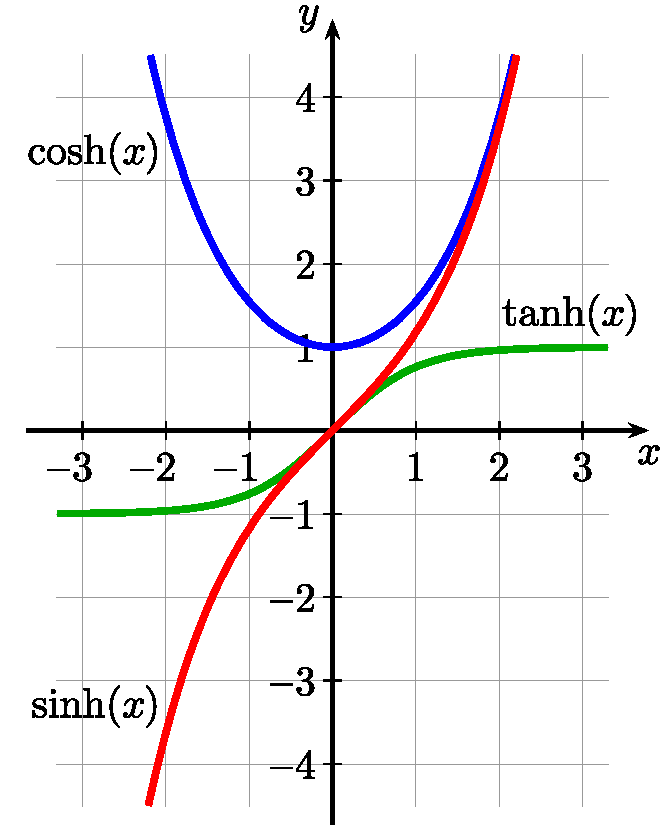
\includegraphics[width = 2cm]{./hyperbolis.pdf} }
\end{sectionbox}

\begin{sectionbox}
	\subsection{holomorphe(analytische, reguläre) Funktionen $\cx f$}
	Eine Funktion $\cx f$ ist \\ 
	\begin{tablebox}{ll}
		holomorph & falls $\cx f$ in $G$ komplex differenzierbar ist.\\
		ganz & falls $\cx f$ in ganz $\C$ komplex differenzierbar ist.\\
		konform & falls Kurven Winkel- und Orientierungstreu bleiben.\\

	\end{tablebox}
	$\cx f$ ist genau dann holomorph, falls $f(x+y\i) = u(x,y) + \i v(x,y)$ und
	\begin{itemize}\itemsep0pt
		\item $u,v$ sind stetig partiell diffbar
		\item Cauchy-Riemann DGLs sind erfüllt:\\
		$\partial_x u(x,y) = \partial_y v(x,y)$ \qquad $\partial_y u(x,y) = - \partial_x v(x,y)$\\
	\end{itemize}
	Holomorph: $\exp, \sin, \cosh$, Polynome, $\cx f\pm \cx g, \cx f \cx g, \frac{\cx f}{\cx g}, \cx f(\cx g)$
\end{sectionbox}

\begin{sectionbox}
	\subsection{harmonische Funktionen $u,v$}
	$u$ bzw. $v$ sind harmonisch, falls gilt:\\
	$\lpo u = \partial_{xx} u + \partial_{yy} u = 0$ \qquad\quad $\lpo v = \partial_{xx} v + \partial_{yy} v = 0$\\[0.5em]
	oder falls $f(\cx z) = u + \i v$ holomorph ist; denn mit Satz von Schwarz:\\
	$\lpo u = \partial_{yx} v - \partial_{xy} v = 0$ \qquad\quad $\lpo v = - \partial_{yx} u + \partial_{xy} u = 0$\\
	\\
	\begin{cookbox}{Bestimmung der harmonischen Konjugierten}
		\begin{itemize}
			\item geg: harm. Fkt. $u: G \ra \mathbb R, (x,y) \ra u(x,y)$
			\item ges: harm. Fkt. $v: G \ra \mathbb R, (x,y) \ra v(x,y)$
			so, dass $f: G \ra \mathbb V, f(z) = u(x,y) + \i v (x,y)$
			\item $v(x,y) = \int u_x \diff y$ mit Integrationskonstante $g(x)$
			\item $v_x = -u_y \Ra g'(x)$
			\item $g(x) = \int g'(x) \diff x \Ra v$ bis auf Konstante $C$ bestimmt
			\item zugehörige holomorphe Fkt.
			$f (z) = u (x,y) + \i v(x,y)$
		\end{itemize}
	\end{cookbox}
\end{sectionbox}

\begin{sectionbox}
%	\subsection{Möbiustransformation $\hat \C = \C \cup \eset{\infty}$}
	Einzige bijektive, holomorphe, konforme Abbildung von $\hat \C$ auf sich selbst.\\
	$\cx f:\C \setminus \eset{-\frac{d}{c}} \ra \C \setminus \eset{-\frac{d}{c}}, \cx f(\cx z) = \frac{a\cx z + b}{c\cx z + d}$ \qquad $ad - bc \ne 0$\\ 
	$\cx f^{-1}(\cx w) = \frac{d\cx w - b}{-c \cx w + a}$
\end{sectionbox}

\begin{sectionbox}
	\subsection{Komplexes Kurvenintegral}
	für $D \subset \mathbb C$ Gebiet, $f: D \ra \mathbb C$ stetig, $\cx \gamma: [t_1, t_2] \ra $ stetig diffbar orientierte Kurve. \\ 
	\begin{cookbox}{So brechnet man ein komplexes Kurvenintegral}
		\item Bestimme Parametrisierung von $\cx \gamma$ \\
		$\cx \gamma = \cx \gamma_1 + \ldots + \cx \gamma_2$, $\cx \gamma_i : [a_i, b_i] \ra \C$
		\item Stelle Inegrale auf \\
		$\int_{\cx \gamma_i} \cx f(\cx z) \diff \cx z = \int \limits_{a_i}^{b_i} \cx f\big(\cx \gamma_i(t)\big) \cdot \dot{\cx \gamma}_i (t) \diff t$\\
		Falls $\cx f$ holomorph: $\int_{\cx \gamma} \cx f(\cx z) \diff \cx z = \cx F\big(\cx \gamma(b)\big) - \cx F\big(\cx \gamma(a)\big)$
		\item Berechne die Integrale und addiere: \\
		$\int \limits_{\cx \gamma} \cx f(z\cx ) \diff \cx z = \sum \limits_{i = 1}^{h} \int_{\cx \gamma_i} \cx f(\cx z) \diff \cx z$
	\end{cookbox}
\end{sectionbox}

\begin{sectionbox}
	\subsection{Cauchy-Integralformel}
	(falls Unstetigkeitsstelle auf Gebiet $G$)
	Falls $\cx \gamma$ geschl. doppelpunktfreie Kurve in einfach zsh. Gebiet $G$ mit holomorphen Fkt. $\cx f$, gilt für jedes $\cx z_0 \in G$\\
	\boxed{\cx f(\cx z_0) = \frac{1}{2\pi \i} \ointctrclockwise_{\cx \gamma} \frac{\cx f(\cx z)}{\cx z - \cx z_0} \diff \cx z }\\
	$\cx f^{(k)}(\cx z_0) = \frac{k!}{2\pi \i} \oint_{\cx \gamma} \frac{\cx f(\cx z)}{(\cx z - \cx z_0)^{k+1}} \diff \cx z$ 
	
	\subsection{Integralsatz von Cauchy}
	Falls keine Unstetigkeitsstelle innerhalb der Kurve $\cx \gamma$\\ 
	$\cx f: G \ra \C$ komplex diffbar auf offenem, einfach zusammenhängendem Gebiet $G \subset \C$. $\cx \gamma$ sei einfach geschlossene Kurve in $G$ (keine Doppelpunkte). \\
	$\oint \limits_{\cx \gamma} \cx f(\cx z) \diff \cx z = 0$
\end{sectionbox}

\begin{sectionbox}
	\subsection{Singularitäten}
	Isolierte Singularität $\cx z_0$: \quad $\cx f :G \setminus \eset{\cx z_0} \ra \C$ \ (einzelne Punkte)\\
	Hebbare Sing., falls $f$ auf punktierter Umgebung beschränkt ist.\\
	Pol $m$ter Ordnung: $(\cx z - \cx z_o)^m \cx f(\cx z)$ ist hebbar in $\cx z_0$\\
	Wesentliche Singularität: Sonst.
\end{sectionbox}

\begin{sectionbox}
	\subsection{Taylorreihe und Laurentreihe}
	\emph{Taylorreihe:} falls $\cx f$ holomorph:\\
	\boxed{ \cx f(\cx z) = \sum\limits_{k = 0}^{\infty} \frac{\cx f^{(k)} \cx z_0}{k!} (\cx z - \cx z_0)^k }\\
	\\
	\emph{Laurentreihe:} Falls $\cx f$ nicht holomorph ist.\\
	\boxed{\sum\limits_{k = -\infty}^\infty \cx c_k (\cx z - \cx z_0)^k} \\
	zerfällt in $\sum \limits_{k=1}^{\infty} d_k w^k$ mit $d_k = c_{-k}$ und $w = \frac{1}{z - z_0}$ (Hauptteil) und $\sum \limits_{k = 0}^{\infty} c_k (z-z_0)^k$ (Nebenteil) \\
	Konvergenz falls Hauptteil und Nebenteil konvergiert. \\ 
	Konvergenzradien: $R = \lim \abs{\frac{c_k}{c_{k+1}}} \in [0, \infty]$ \\ 
	Resiudensatz: $\mathrm{Res}_{z_0} \cx f = c_{-1} = \frac{1}{2\pi\i} \oint f(z) \diff z$
	
	\paragraph{Allgemeiner Residuensatz} $G$ Gebiet: $f:G \setminus \eset{z_1, \ldots, z_n} \ra \mathbb C$ hol. \\ 
	$\forall $ doppelpunktfrei, geschlossene und pos. orientierte Kurven $\gamma$ mit $z_1, \ldots z_n$ liegen im Inneren von $\gamma$: \\ 
	$\oint_\gamma f(z) \diff z = 2 \pi \i \sum_{k=1}^{n} Res_{z_k} f$
	
	\begin{emphbox}
		\raggedright
		$\mathrm{Res}_{\cx z_0} \frac{\cx g}{\cx h} = \frac{\cx g(\cx z_0)}{\cx h'(\cx z_0)}$ \qquad $\mathrm{Res}_{\cx z_0} \frac{\cx g(\cx z)}{(\cx z - \cx z_0)^m} = \frac{\cx g^{(m-1)}(\cx z_0)}{(m-1)!}$\\
		$\mathrm{Res}_{\cx z_0} \cx g \frac{\cx h'}{\cx h} = m \cx g(\cx z_0)$ \qquad $m:$ Ordnung der Polstelle
	\end{emphbox}
\end{sectionbox}




% Dokumentende
% ======================================================================
\end{document}